\section{Theorie} \label{sec:Theorie}

\subsection{Grundlegendes Prinzip der Wärmepumpe}

    Die Wärmepumpe wird dazu verwendet, die Richtung des Wärmeflusses umzukehren.
    Der \enquote{natürliche} Wärmefluss findet in einem abgeschlossenen System von einem heißeren Körper zu einem kälteren Körper statt.

    Um die Richtung des Wärmeflusses umzukehren,
    muss (hier: mechanische) Arbeit aufgewendet werden.
    Nach dem ersten Hauptsatz der Thermodynamik ist dabei die abgegebene Temperatur $Q_1$ vom heißeren Körper gleich der aufgenommenen Wärme $Q_2$ des kälteren Körpers und der benötigten Arbeit $A$.
    Es gilt also:
    \begin{equation*}
        Q_1 = Q_2 + A \; .
    \end{equation*}

    Mit der Beziehung zwischen Wärme und Temperatur im realistischen, irreversiblen Fall
    \begin{equation*}
        \frac{Q_1}{T_1} - \frac{Q_2}{T_2} > 0
    \end{equation*}
    ergibt sich außerdem:
    \begin{equation*}
        Q_1 = A + \frac{T_1}{T_2} Q_2 \; .
    \end{equation*}

    Das Verhältnis zwischen der abgegebenen Wärme $Q_1$ und der benötigten mechanischen Arbeit $A$ wird durch die Güteziffer $\nu$ beschrieben:
    \begin{equation*}
        \nu = \frac{Q_1}{A} \; .
    \end{equation*}


\subsubsection{Bestimmung der realen Güteziffer}
% \label{sec:reale_gueteziffer}

    Die mechanische Arbeit kann auch durch ein Zeitintervall und die Leistungsaufnahme $N$ des Kompressors ausgedrückt werden:
    \begin{equation*}
        \nu_\text{real} = \frac{\symup{\Delta} Q_1}{\symup{\Delta} t N} \; .
    \end{equation*}

    Der Quotient $\frac{\symup{\Delta} Q_1}{\symup{\Delta} t}$ beschreibt hier die pro Zeiteinheit gewonnene Wärmemenge.

    Es gilt
    \begin{equation*}
        \frac{\symup{\Delta} Q_1}{\symup{\Delta} t} = (m_1 c_\text{w} + m_\text{k} c_\text{k}) \frac{\symup{\Delta} T_1}{\symup{\Delta} t}
    \end{equation*}
    und somit auch
    \begin{equation}
      \label{eqn:reale_gueteziffer}
      \nu_\text{real} = \frac{1}{N} (m_1 c_\text{w} + m_\text{k} c_\text{k}) \frac{\symup{\Delta} T_1}{\symup{\Delta} t} \; .
    \end{equation}


\subsubsection{Bestimmung des Massendurchsatzes}
\label{sec:massendurchsatz}

    Die aus dem Reservoir 2 entnommene Wärmemenge wird durch
    \begin{equation*}
        \frac{\symup{\Delta} Q_2}{\symup{\Delta} t}
        = (m_2 c_\text{w} + m_\text{k} c_\text{k}) \frac{\symup{\Delta} T_2}{\symup{\Delta} t}
    \end{equation*}
    beschrieben.

    Wenn die Verdampfungswärme $L$ bekannt ist, lässt sich der Massendurchsatz aus
    \begin{equation*}
        \frac{Q_2}{\symup{\Delta} t} = L \frac{\symup{\Delta} m}{\symup{\Delta} t}
    \end{equation*}
    bestimmen.

    Tatsächlich muss $L$ noch bestimmt werden, was durch Berechnung einer linearen Regression geschieht.
    Als Ansatz dient die Approximation der Clausius-Clapeyron-Gleichung für ein ideales Gas.
    $L$ bezeichnet dabei die (molare) Verdampfungswärme, und $R$ ist die universelle Gaskonstante.

    \begin{align*}
      \frac{1}{p} \mathrm{d}p &= \frac{L}{R \cdot T^2} \mathrm{d} T \\
      \ln(p) &= \frac{L}{R} \cdot \frac{1}{T} + c \\
      % \mathrm{ln}(p) &= \frac{L}{R \cdot T} + c \\
      % \mathrm{ln}(p) \cdot (R \cdot T) &= L + c \\
    \end{align*}

    Durch Integration wurde eine Form gefunden,
    mit der $\frac{L}{R}$ die Steigung $a$ der Regressionsgeraden ist,
    wenn $\ln(p)$ gegen $\frac{1}{T}$ aufgetragen wird.
    Also ist $L = a \cdot R$.

    Schließlich wird aus der molaren Verdampfungswärme $L$
    die Verdampfungswärme mit Bezug auf eine Masse berechnet,
    indem durch die molare Masse $M$ dividiert wird:
    \begin{equation*}
      L_\text{Masse} = \frac{L}{M}
      \; .
    \end{equation*}

\subsubsection{Bestimmung der mechanischen Kompressorleistung}

    Die Arbeit $A_\text{m}$, die benötigt wird,
    um das Gasvolumen $V_\text{a}$ auf den Wert $V_\text{b}$ zu verringern,
    wird durch
    \begin{equation*}
        A_\text{m} = - \displaystyle\int_{V_\text{a}}^{V_\text{b}} p dV
    \end{equation*}
    bestimmt.

    Zudem ergibt sich die Poisson'sche Gleichung als Zusammenhang zwischen Druck und Volumen
    \begin{equation*}
        p_\text{a} V_\text{a}^\text{\kappa} = p_\text{b} V_\text{b}^\text{\kappa} = p V^\text{\kappa} \; .
    \end{equation*}

    Für $A_\text{m}$ ergibt sich damit
    \begin{equation*}
       A_\text{m} = - p_\text{a} V_\text{a}^\text{\kappa} \displaystyle\int_{V_\text{a}}^{V_\text{b}} V^{-\kappa} dV
                  = \frac{1}{\kappa - 1} p_\text{a} V_\text{a}^\text{\kappa} (V_\text{b}^{-\kappa+1} - V_\text{a}^{-\kappa+1})
                  = \frac{1}{\kappa - 1} \left(p_\text{b} \sqrt[\kappa]{\frac{p_\text{a}}{p_\text{b}}} - p_\text{a}\right) V_\text{a} \; .
    \end{equation*}

    Außerdem gilt für die mechanische Kompressorleistung mit der Beziehung $V_\text{a} = \frac{1}{\rho} m$
    \begin{equation}
      \label{eqn:N_mech}
        N_\text{mech} = \frac{\symup{\Delta} A_\text{m}}{\symup{\Delta} t}
                      = \frac{1}{\kappa-1} \left(p_\text{b} \sqrt[\kappa]{\frac{p_\text{a}}{p_\text{b}}} - p_\text{a}\right) \frac{1}{\rho} \frac{\symup{\Delta} m}{\symup{\Delta} t} \; .
    \end{equation}

    Hierbei bezeichnet $\rho$ die Dichte des Gases im gasförmigen Zustand.
    Die Variable $\kappa$ bezeichnet das Verhältnis der Molwärmen und ist immer positiv.


\subsection{Aufbau einer Wärmepumpe}
\label{sec:Aufbau}

    \begin{figure}
      \centering
      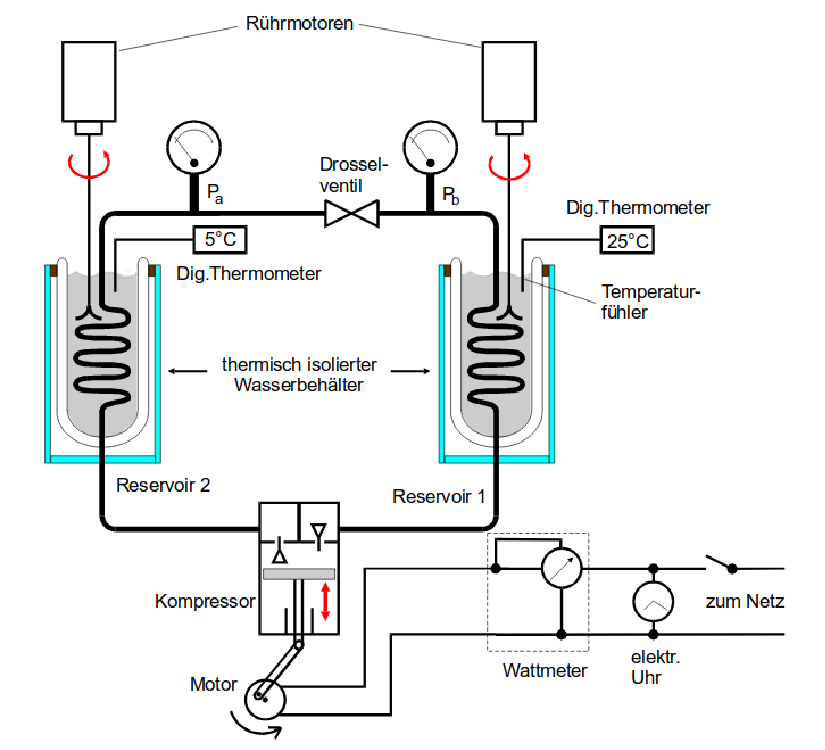
\includegraphics[scale=0.8]{content/img/aufbau.pdf}
      \caption{Schematischer Aufbau einer Wärmepumpe.}
      \label{fig:aufbau}
    \end{figure}

    % TODO: Mehr Bezug auf das Bild nehmen

    Der grundsätzliche Aufbau der Wärmepumpe besteht aus zwei unterschiedlich warmen Reservoiren und einem Kompressor $K$,
    der das Wärmetransportmedium durch die Kompression erhitzt.
    Um die Wärme zwischen den Reservoiren 1 und 2 zu transportieren,
    wird ein Gas verwendet,
    welches beim Wechsel in den gasförmigen
    Aggregatzustand Wärme aufnimmt und sie wieder abgibt,
    sobald es wieder flüssig wird.

    Der Kompressor stellt einen Mediumkreislauf in der Wärmepumpe her.
    Zwischen den Reservoiren herrscht ein hoher Druckunterschied,
    welcher durch ein Drosselventil $D$ erzeugt wird.
    Bei einem Druck $p_1$ (in der Abbildung $P_b$) und einer Temperatur $T_1$ aus dem ersten Reservoir ist das Gas flüssig,
    bei einem Druck $p_2$ (in der Abbildung $P_a$) und einer Temperatur $T_2$ aus dem zweiten Reservoir ist das Gas gasförmig.

    Das Gas wird zu Beginn des Kreislaufs im Kompressor $K$ stark erhitzt und durchläuft anschließend das erste Reservoir.
    Hier wird dem Gas Wärme entzogen und es wird flüssig.
    Somit ist das erste Reservoir das Wärmenehmende.
    Danach durchläuft das Gas das Drosselventil $D$,
    wobei ein Reiniger $R$ das flüssige Medium von Blasenresten trennt,
    um den Kompressor nicht zu beschädigen.
    Die Durchlässigkeit wird hier durch den Temperaturunterschied zwischen $T_1$ und $T_2$ gesteuert.
    Im zweiten Reservoir nimmt das Gas wieder Wärme auf und wird gasförmig.
    Somit ist das zweite Reservoir das Wärmeabgebende.
    Das Gas gelangt zurück in den Kompressor und wird wieder erhitzt.
